\section{Reduced Order Modeling}
\label{sec:ROMs}
The development of high-fidelity codes, for thermal-hydraulic systems
and integrated multi-physics, has undergone a significant acceleration
in the last years. Multi-physics codes simulate
multiple physical models or multiple simultaneous physical phenomena,
in a integrated solving environment. Multi-physics typically
solves coupled systems of partial differential equations, generally
characterized by several different geometrical and time scales.

The new multi-physics codes are characterized by remarkable
improvements
in the approximation of physics (high approximation order and reduced
use of empirical correlations). This greater fidelity is generally
accompanied by a greater computational effort (calculation time
increased). This peculiarity is an
obstacle in the application of  computational techniques of
quantification of uncertainty and risk associated with the operation of
particular industrial plant (e.g., a nuclear reactor).

A solution to this problem is represented by the
usage
of highly effective sampling strategies. Sometimes also these
approaches is not enough
in order to perform a comprehensive UQ and PRA analysis. In these
cases the help of reduced order modeling is essential.

RAVEN has support of several different ROMs,
such as:
\begin{enumerate}
  \item \textit{Nearest Neighbors approaches}
  \item \textit{Support Vector Machines}
  \item \textit{Inverse Weight regressors}
  \item \textit{Spline regressors }, etc.
\end{enumerate}
In this section only few of them are going to be analyzed, explaining the theory behind it
by way of applied RAVEN examples.

A ROM, also known a surrogate
model, is a mathematical representation of a system, used to predict
a FOM of a physical system.

The ``training'' is a process of setting the internal parameters of the ROM from a set
of samples generated the physical model, .e.,
 the high-fidelity simulator (RELAP-7, RELAP5
3D, PHISICS, etc.),
\begin{figure}[h!]
  \centering
  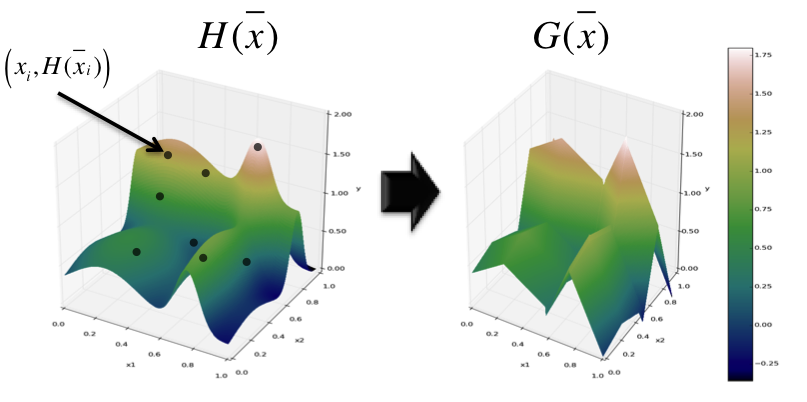
\includegraphics[width=1.0\textwidth]  {pics/ROMexampleOfPhysicalSystem.png}
  \caption{Example of reduced order model representation of physical system (regression).}
  \label{fig:ROMexampleOfPhysicalSystem}
\end{figure}

Two characteristics of these models
are generally assumed (even if exceptions are possible):
\begin{enumerate}
  \item The higher the number of realizations in the training sets, the
higher is the accuracy of the prediction performed by the ROM is. This
statement is true for most of the cases, although some ROMs might be
subject to the over-fitting issues. The over-fitting phenomenon is not
analyzed in this thesis, since its occurrence highly depends on the
algorithm type, and, hence, the problem needs to be analyzed for all
the large number of ROM types available;
  \item The smaller the size of the input (uncertain) domain with
  respect to the variability of the system response, the more likely the
  ROM is able to represent the system response space.
\end{enumerate}

\subsection{Reduced Order Modeling: Theory}
\label{sec:ROMsTheory}
To provide a very simple idea of a ROM, assume that the final
response space of a physical system is governed by the transfer
function $H \left (  \overline{x}\right)$ (see Section
~\ref{sub:mathBackground}), which, from a practical point of
view, represents the outcome of the system based on the initial
conditions  $\overline{x}$. Now, sample the domain of variability of the
initial conditions $\overline{x}$ to create a
set of $N$ realizations of the input and response space $ \left ( \left (
\overline{x}_{i}, H \left (  \overline{x}_{i}\right) \right), i=1,N \right)$,
named ``training'' set. Based on the data set generated, it is possible
to construct a mathematical representation $G\left ( \overline{x}:
\overline{x}_{i}\right)$ of the
real system $H \left (  \overline{x}\right)$, which will approximate its
response (see Figure~\ref{fig:ROMexampleOfPhysicalSystem}):
\begin{equation}
\label{eq:regressor}
G\left ( \overline{x} \right ):\overline{x}_{i} \rightarrow G\left ( \overline{x}_{i} \right ) \cong H\left ( \overline{x}_{i} \right )
\end{equation}
The ROMs reported above are generally named ``regressors'', among
which all the most common data fitting algorithms are found (e.g.,
least square for construction of linear models).

An important class of ROMs for the work presented here after is the
one containing the so called ``classifiers''. A classifier is a ROM that is
capable of representing the system behavior from a binary point of
view (e.g., event happened/not happened or failure/success). It is a
model (set of equations) that identifies to which category an object
belongs in the feature (input) space. Referring to the example that
brought to Equation ~\ref{eq:regressor}, a classifier can be formally represented as follows (see
Figure~\ref{fig:ROMClassifierExampleOfPhysicalSystem}):
\begin{figure}[h!]
  \centering
  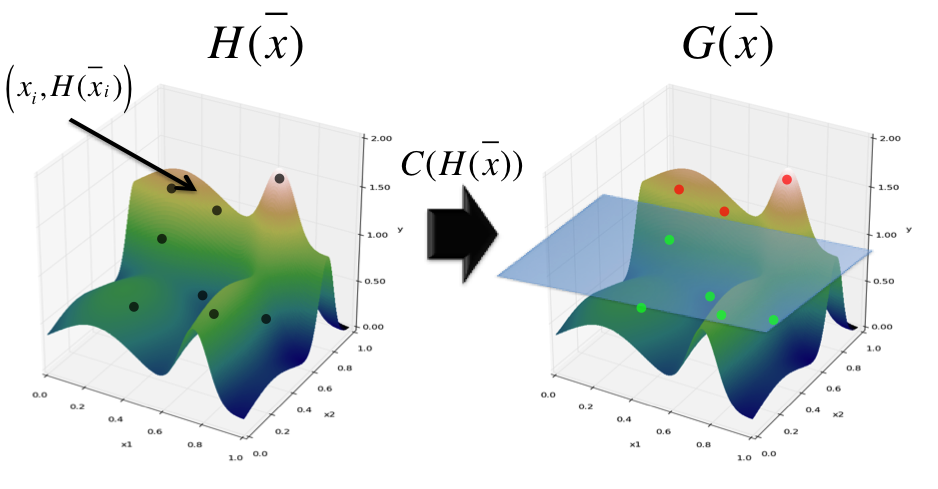
\includegraphics[width=1.0\textwidth]  {pics/ROMClassifierExampleOfPhysicalSystem.png}
  \caption{Example of reduced order model representation of physical system (classifier).}
  \label{fig:ROMClassifierExampleOfPhysicalSystem}
\end{figure}

\begin{equation}
\label{eq:classifier}
G\left ( \overline{x} \right ):\overline{x}_{i} \rightarrow G\left ( \overline{x}_{i} \right ) \cong
C \left ( H\left ( \overline{x}_{i} \right ) \right )
\end{equation}

The function $C\left (  H\left ( \overline{x}_{i}  \right ) = \overline{\theta}
\right ) $ is the so called ``goal'' function that is able to recast the
response of the system $H\left ( \overline{x}_{i}  \right )$ into a binary
form (e.g., failure/success). As an example, referring to
Figure~\ref{fig:ROMClassifierExampleOfPhysicalSystem}, the
``goal'' function would be:
\begin{equation}
\label{eq:goalFunctionClassifier}
C\left (   \overline{\theta}  \right ) = \left\{\begin{matrix}
1 & if \: \overline{\theta}>1.0 \\
0 &  if \: \overline{\theta} \leq 1.0
\end{matrix}\right.
\end{equation}
Hence, the ROM of type classifier $G\left (  \overline{x} \right )$  will operate in the space transformed through the ``goal''  function $C\left (   \overline{\theta}  \right )$.
\\The classifiers and regressors can be categorized into two main classes:
\begin{itemize}
  \item Model-based algorithms
  \item Data-based algorithms
\end{itemize}
In the first class, the created ROM aims to approximate the response
of the system as a function of the input parameters. These algorithms
construct a functional representation of the system. Examples of such ROM type are Support Vector Machines (SVMs), Kriging-based regressors, discriminant-based models, and polynomial chaos.

On the other side, data-based algorithms do not build a response-
function-based ROM but classify or predict the response of the
system from the neighborhood graph constructed from the training
data, without any dependencies on a particular prediction model.
These algorithms directly build a neighborhood structure as the
ROM (e.g., a relaxed Gabriel graph) on the initial training data. Examples of such ROM type are nearest neighbors and decision trees.

\textcolor{red}{\\It is important to NOTICE that RAVEN uses a Z-score normalization of the training data before 
  constructing most of the ROMs:
\begin{equation}
  \mathit{\mathbf{X}} = \frac{(\mathit{\mathbf{X}}-\mu )}{\sigma }
\end{equation} 
 } 
In order to understand which ROMs get trained with data normalized by the previous reported normalization approach, please refer to the RAVEN user manual \cite{RAVENuserManual}.

\subsubsection{Gaussian Process Models}
\label{sec:GPM}
Gaussian Processes (GPs)~\cite{Rasmussen_GPM} are algorithms that extend multivariate Gaussian distributions to infinite dimensionality. A Gaussian process generates a data set located throughout some domain such that any finite subset of the range follows a multivariate Gaussian distribution. Now, the n observations in an arbitrary data set, $y={y_1,\ldots,y_n}$, can always be imagined as a single point sampled from some multivariate ($n$-variate) Gaussian distribution.
What relates one observation to another in such cases is just the covariance function, $k(x,x')$. A popular choice is the squared exponential:
\begin{equation}
k(x,x')=\sigma_{f}^{2}  exp \left [ \frac{-(x-x')^2}{2 l^2} \right ]
\end{equation}
where the maximum allowable covariance is defined as $\sigma_{f}^{2}$; this should be high for functions that cover a broad range on the y axis. If $x \simeq x'$, then $k(x,x')$ approach this maximum meaning $f(x)$ is very correlated to $f(x')$. On the other hand, if $x$ is very distant from $x'$, then $k(x,x' ) \simeq 0$ (i.e., the two points cannot see each other.
So, for example, during interpolation at new $x$ values, distant observations will have negligible effect). How much effect this separation has will depend on the length parameter $l$.
Each observation $y$ can be thought of as related to an underlying function $f(x)$ through a Gaussian noise model:
\begin{equation}
y=f(x)+N(0,\sigma_{n}^{2})
\end{equation}
The new kernel function can be written as:
\begin{equation}
k(x,x')=\sigma_{f}^{2}  exp \left [ \frac{-(x-x')^2}{2 l^2} \right ] + \sigma_{n}^{2} \delta(x,x')
\end{equation}
So given $n$ observations $y$, the objective is to predict the value $y_*$ at the new point $x_*$. This process is performed by following this sequence of steps:
\begin{enumerate}
\item Calculate three matrices:
\begin{equation}
K=\begin{bmatrix}
k(x_1,x_1) &  \ldots & k(x_1,x_n)\\
\vdots  & \ddots &\vdots  \\
k(x_n,x_1) &  \ldots & k(x_n,x_n)
\end{bmatrix}
\end{equation}
\begin{equation}
K_*= \begin{bmatrix}
k(x_*,x_1) & \ldots & k(x_*,x_n)
\end{bmatrix}
\end{equation}
\begin{equation}
K_{**}=k(x_*,x_*)
\end{equation}
\item The basic assumption of GPM is that:
\begin{equation}
\begin{bmatrix}
y\\
y_*
\end{bmatrix}
=\mathcal{N}(0,\begin{bmatrix}
K & K_{*}^{T}\\
K_* & K_{**}
\end{bmatrix})
\end{equation}
\item The estimate $\bar{y_*} $ for $y_*$ is the mean of this distribution
\begin{equation}
\bar{y_*}=K_* K^{-1}y
\end{equation}
\item The uncertainty associated to the estimate $\bar{y_*} $ can be expressed in terms of variance of  $y_*$:
\begin{equation}
var(y_*)=K_{**}-k_* K^{-1} K_{*}^{T}
\end{equation}
\end{enumerate}

\subsubsection{Support Vector Machines}
\label{sec:SVM}
The Support Vector Machine (SVM)~\cite{SVM_Burges} classifier is a methodology that aims to determine the optimal separation hyperplane between data sets having different labels.
The training data consist of $N$ data points $(x_i,y_i)$ $i=1,\ldots,N$ where $x_i \in \mathbb{R}^M$ and $y_i \in {-1,1}$.
Assuming a linear property of the hyperplane  then its definition is:
\begin{equation}
\left \{ x: f(x)=x^T\beta+\beta_0=0 \right \}
\end{equation}
where $\beta$ is a unit vector.

The SVM parameters $\beta$ and $\beta_0$  are determined by solving this optimization problem:
\begin{equation}
\left\{\begin{matrix}
\underset{\beta,\beta_0}{min} \left \| \beta \right \|\\
\text{subject to } y_i(x_{i}^{T}\beta+\beta_0)\geq 1 , \quad i=1,\dots,N
\end{matrix}\right.
\end{equation}

Once the SVM parameters $\beta$ and $\beta_0$ are determined then the classification of a new point $\bar{x}$ is given by:
\begin{equation}
G(\bar{x})=sign(\bar{x}^T\beta+\beta_0)
\end{equation}


\subsubsection{KNN Classifier and KNR Regressor}
\label{sec:KNN_KNR}
The K Nearest Neighbor algorithm~\cite{altman_KNN} (KNN) is a non-parametric method used for both regression and classification. The only input parameter is the variable $K$ which indicates the number of neighbors to be considered in the classification/regression process. The special case where the class is predicted to be the class of the closest training sample (i.e. when $K = 1$) is called the nearest neighbor algorithm. In binary (two class) classification problems, it is helpful to choose k to be an odd number as this avoids tied votes. The output depends on whether KNN is used for classification or regression:
\begin{itemize}
\item In KNN classification, the output is a class membership. An object is classified by a majority vote of its neighbors, with the object being assigned to the class most common among its $K$ nearest neighbors ($K$ is a positive integer, typically small). If $K = 1$, then the object is simply assigned to the class of that single nearest neighbor.
\item In KNN regression, the output is the property value for the object. This value is the average of the values of its $K$ nearest neighbors.
\end{itemize}
Both for classification and regression, it can be useful to assign weight to the contributions of the neighbors, so that the nearer neighbors contribute more to the average than the more distant ones. For example, a common weighting scheme consists in giving each neighbor a weight of $1/d$, where $d$ is the distance to the neighbor.

\subsubsection{Multi-Dimensional Interpolation}
\label{sec:ND_interp}
This section covers the methods that have been implemented in the CROW statistical library:
\begin{itemize}
\item Shepard's Method (see Section~\ref{sec:shepard})
\item Multi-Dimensional Spline method (see Section~\ref{sec:ND_spline}).
\end{itemize}

These two methods are interpolation methods that can be used in any dimension.
In RAVEN they are employed in two major applications:
\begin{enumerate}
\item ROMs
\item Multi-dimensional distributions.
\end{enumerate}
For both applications, given a set of $N$ data points $ (x_i,u_i )$  $i=1,\ldots,N$ where $x_i$ are the coordinate in the input space $D \subset \mathbb{R}^M$ and $u_i \in \mathbb{R}$ is the outcome, the methods predicts the outcome $\tilde{u}$ for a new coordinate $\tilde{x}\in \mathbb{R}^n$.


\paragraph{Shepard's Method}
\label{sec:shepard}
The Shepard interpolator~\cite{Shepard} is also know as Inverse Distance Weighting (IDW) interpolator.
The starting point is a set of $N$ data points $ (x_i,u_i )$ for $i=1,\ldots,N$.
The Inverse-Weight interpolator can be represented as a function $f_{IDW}(x)$ that, given a new coordinate in the input space $x$, generates a prediction on $u$ such that
\begin{equation}
u:x \in \mathbb{R}^M \rightarrow f_{IDW}(x) \in \mathbb{R}
\end{equation}
based on the distance $d(x,x_i)$ in the euclidean space between $x$ and $x_i$.

Such prediction $u=f_{IDW}(x)$ is performed by summing all data points $x_i$ $i=1,\ldots,N$ weighted by a weighting parameter $w_i (x)$ as follows:
\begin{equation}
f_{IDW}(x) =
\left\{
\begin{matrix}
\sum_{i=1}^{N} w(x_i) u_i &  \text{if } d(x,x_i) \neq 0 \\
 u_i &  \text{if } d(x,x_i) = 0
\end{matrix}\right.
\end{equation}
where
\begin{equation}
w(x_i) =\frac{w_i}{\sum_{i=1}^{N} w_i}
\end{equation}
and
\begin{equation}
w_i = \left ( \frac{1}{d(x,x_i)} \right )^p
\end{equation}
Large values of $p$ assign greater weight $w_i$ to data points $x_i$ closest to $x$, with the result turning into a mosaic of tiles (i.e., Voronoi diagram) with nearly constant interpolated value.

\paragraph{Multi-Dimensional Spline}
\label{sec:ND_spline}
The Multi-Dimensional Spline (MDS)~\cite{MD_spline} is a method that requires the sampled points $x_i$ to be lying in multi-dimensional cartesian grid.
A generic grid $\Delta_m$ for each dimension $m$ will be indicated as follows:
\begin{equation}
\Delta_m = \{x_{0_m},x_{1_m},\ldots,x_{p_m}\} \text{ for } m=1,\ldots,M
\end{equation}
This methods construct a $M$-dimensional cubic spline so that, given a coordinate in the input space $x=(x_1,x_2,\ldots,x_M)$, generates a prediction on $u$ such that
\begin{equation}
u:x \in \mathbb{R}^M \rightarrow f_{MDS}(x) \in \mathbb{R}
\end{equation}
where
\begin{equation}
f_{MDS}(x)=\sum_{i_1=1}^{p_1+3} \sum_{i_2=1}^{p_2+3} \ldots \sum_{i_M=1}^{p_M+3} c_{i_1,i_2,\ldots,i_p} \prod_{m=1}^{M} u_{i_j} (x_m)
\end{equation}
where
\begin{equation}
u_{i_j} (x_m) = \Phi\left ( \frac{x_m-x_{0_m}}{h_j}+2-i_j  \right )
\end{equation}

The cubic kernel $\Phi(t)$ is defined as:
\begin{equation}
\Phi(t) = \left\{\begin{matrix}
(2-\left | t \right |)^3 & 1\leq \left | t \right |\leq 2 \\
4-6\left | t \right |^2+3\left | t \right |^3 & \left | t \right |\leq 1\\
0 & \text{elsewhere}
\end{matrix}\right.
\end{equation}

The set of $\prod_{m=1}^{M}(p_m+3)$ coefficients $c_{i_1,i_2,\ldots,i_p}$  is determined when the interpolator is initialized.

%%%%%%%%%%%%%%%%
\subsection{Reduced Order Modeling through RAVEN}
\label{subsub:ROMraven}
The goals of this section are about learning how to:
 \begin{enumerate}
   \item Set up a sampling strategy to construct multiple ROMs, perturbing a driven code
   \item Train the different ROMs with the data-set obtained by the applied sampling strategy;
   \item Use the same sampling strategy, perturbing the ROMs
   \item Plot the responses of the driven code and ROMs, respectively.
\end{enumerate}
In order to accomplish these tasks, the following RAVEN \textbf{Entities} (XML blocks in the input files) need to be defined:
\begin{enumerate}
   \item \textbf{\textit{RunInfo}}:
\begin{lstlisting}[style=XML,morekeywords={arg,extension,pauseAtEnd,overwrite}]
  <RunInfo>
    <JobName>Chapter-IX/ROMConstruction</JobName>
    <Sequence>
        sample,trainROMGaussianProcess,trainROMsvm,
        trainROMinverse,sampleROMGaussianProcess,
        sampleROMInverse,sampleROMsvm,writeHistories
    </Sequence>
    <WorkingDir>ROMConstruction</WorkingDir>
    <batchSize>12</batchSize>
  </RunInfo>
\end{lstlisting}
   As in the other examples, the the \textit{RunInfo} \textbf{Entity} is intended  to set up the analysis sequence that
   needs to be performed. In this specific case, eight steps  (\xmlNode{Sequence}) are going to be sequentially run
   using eight processors (\xmlNode{batchSize}).
   \\In the first step, the original physical model is going to be sampled. The obtained results are going to be used to
   train three different ROMs.These ROMs are sampled by the same strategy used in the first step in order to compare the
   ROMs' responses with the ones coming from the original physical model.
   \item \textbf{\textit{Files}}:
\begin{lstlisting}[style=XML,morekeywords={arg,extension,pauseAtEnd,overwrite}]
  <Files>
    <Input name="referenceInput.xml" type="input">referenceInput.xml</Input>
  </Files>
\end{lstlisting}
   Since the driven code uses a single input file, the original input is placed in this section. As detailed in the user manual
   the attribute  \xmlAttr{name} represents the alias that is going to be
   used in all the other input blocks in order to refer to this file.
   \item \textbf{\textit{Models}}:
\begin{lstlisting}[style=XML,morekeywords={arg,extension,pauseAtEnd,overwrite}]
  <Models>
    <Code name="testModel" subType="GenericCode">
      <executable>
       ../physicalCode/analyticalbateman/AnalyticalDplMain.py
      </executable>
      <clargs arg="python" type="prepend"/>
      <clargs arg="" extension=".xml" type="input"/>
      <clargs arg="" extension=".csv" type="output"/>
      <prepend>python</prepend>
    </Code>
    <ROM name="ROMGaussianProcess" subType="SciKitLearn">
      <Features>sigma-A,sigma-B,decay-A,decay-B</Features>
      <Target>A,B</Target>
      <SKLtype>GaussianProcess|GaussianProcess</SKLtype>
      <regr>quadratic</regr>
      <theta0>10</theta0>
    </ROM>
    <ROM name="ROMsvm" subType="SciKitLearn">
      <Features>sigma-A,sigma-B,decay-A,decay-B</Features>
      <Target>A,B</Target>
      <SKLtype>svm|SVR</SKLtype>
      <kernel>rbf</kernel>
      <C>50.0</C>
      <tol>0.000001</tol>
    </ROM>
    <ROM name="ROMinverse" subType="NDinvDistWeight">
      <Features>sigma-A,sigma-B,decay-A,decay-B</Features>
      <Target>A,B</Target>
      <p>3</p>
    </ROM>
  </Models>
\end{lstlisting}
 As mentioned above, the goal of this example is the employment of
 a sampling strategy in order to construct multiple types of ROMs.
 \\Indeed, in addition to the previously explained Code
 model,
 three different ROMs (GP, SVM and IDW) are here specified. The ROMs will be
 constructed (``trained'') through the data-set generated by the sampling of the physical model. Once trained, they are going
 to be used in place of the original physical model.
 \\As it can be seen,
 the ROMs will be constructed considering four features ($sigma-A,\,sigma-B,\, decay-A \,,and \, decay-B$) and two targets
 ($A \, and \, B$).
   \item \textbf{\textit{Distributions}}:
\begin{lstlisting}[style=XML]
  <Distributions>
      <Uniform name="sigma">
          <lowerBound>0</lowerBound>
          <upperBound>1000</upperBound>
      </Uniform>
      <Uniform name="decayConstant">
          <lowerBound>0.00000001</lowerBound>
          <upperBound>0.0000001</upperBound>
      </Uniform>
  </Distributions>
\end{lstlisting}
  In the Distributions XML section, the stochastic model for the
  uncertainties are reported. In
  this case two distributions are defined:
  \begin{itemize}
    \item $sigma \sim \mathbb{U}(0,1000)$, used to model the uncertainties
    associated with  the Model \textit{sigma-A} and \textit{sigma-B};
    \item  $decayConstant \sim \mathbb{U}(1e-8,1e-7)$,  used to
    model the uncertainties
    associated with  the Model \textit{decay-A} and \textit{decay-B}.
  \end{itemize}
   \item \textbf{\textit{Samplers}}:
\begin{lstlisting}[style=XML,morekeywords={arg,extension,pauseAtEnd,overwrite}]
  <Samplers>
    <Grid name="grid">
      <variable name="sigma-A">
        <distribution>sigma</distribution>
        <grid construction="equal" steps="5" type="CDF">0.01 0.99</grid>
      </variable>
      <variable name="decay-A">
        <distribution>decayConstant</distribution>
        <grid construction="equal" steps="5" type="CDF">0.01 0.99</grid>
      </variable>
      <variable name="sigma-B">
          <distribution>sigma</distribution>
          <grid construction="equal" steps="5" type="CDF">0.01 0.99</grid>
      </variable>
      <variable name="decay-B">
          <distribution>decayConstant</distribution>
          <grid construction="equal" steps="5" type="CDF">0.01 0.99</grid>
      </variable>
    </Grid>
  </Samplers>
\end{lstlisting}
  To obtain the data-set through which the ROMs are going to be
  constructed, a \textit{Grid} sampling approach is here employed.
   \item \textbf{\textit{DataObjects}}:
\begin{lstlisting}[style=XML,morekeywords={arg,extension,pauseAtEnd,overwrite}]
  <DataObjects>
    <PointSet name="samples">
      <Input>sigma-A,sigma-B,decay-A,decay-B</Input>
      <Output>A,B,C,D</Output>
    </PointSet>
    <HistorySet name="histories">
        <Input>sigma-A,sigma-B,decay-A,decay-B</Input>
        <Output>A,B,C,D,time</Output>
    </HistorySet>
    <PointSet name="inputPlaceHolder">
      <Input>sigma-A,sigma-B,decay-A,decay-B</Input>
      <Output>OutputPlaceHolder</Output>
    </PointSet>
    <PointSet name="samplesGP">
      <Input>sigma-A,sigma-B,decay-A,decay-B</Input>
      <Output>A,B</Output>
    </PointSet>
    <PointSet name="samplesInverse">
      <Input>sigma-A,sigma-B,decay-A,decay-B</Input>
      <Output>A,B</Output>
    </PointSet>
    <PointSet name="samplesSVM">
      <Input>sigma-A,sigma-B,decay-A,decay-B</Input>
      <Output>A,B</Output>
    </PointSet>
  </DataObjects>
\end{lstlisting}
  Int this block, six \textit{DataObjects} are defined: 1) PointSet
  named ``samples'' used to collect the final outcomes of the code, 2)
  HistorySet named ``histories'' in which the full time responses of the
  variables $A,B,C,D$ are going to be stored, 3) PointSet named
  ``inputPlaceHolder'' used in the \textit{role} of \xmlNode{Input} for the ROMs sampling;
  4) PointSet named ``samplesGP'' used to collect the final outcomes (sampling) of the GP ROM;
  5) PointSet named ``samplesInverse'' used to collect the final outcomes (sampling) of the IDW ROM;
  6) PointSet named ``samplesSVM'' used to collect the final outcomes (sampling) of the SVM ROM.
 %%%%%%%%%%%%%%%%%%%%%%%%%%%%%%%%%%%%%%%%%%%%%%%%%%%%%%%%%%
 %%%%%%%%%%%%%%%%%%%%%%%%%%%%%%%%%%%%%%%%%%%%%%%%%%%%%%%%%%
 %figure samples
 \begin{figure}[h!]
  \centering
  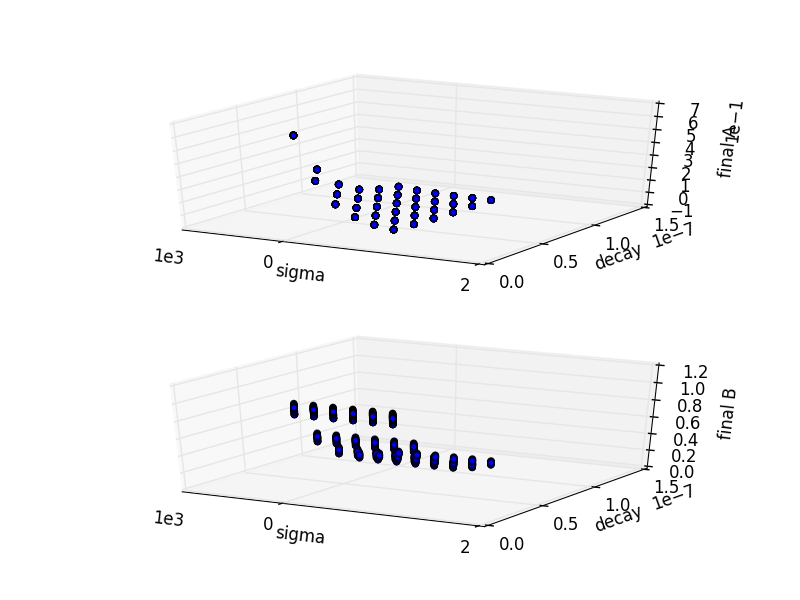
\includegraphics[scale=0.7]{pics/samplesplot3d.png}
  \caption{Plot of the samples generated by the Grid sampling for variables $A,B$.}
  \label{fig:ROMgrid_pointsets}
 \end{figure}
 %%%%%%%%%%%%%%%%%%%%%%%%%%%%%%%%%%%%%%%%%%%%%%%%%%%%%%%%%%
 %%%%%%%%%%%%%%%%%%%%%%%%%%%%%%%%%%%%%%%%%%%%%%%%%%%%%%%%%%
   \item \textbf{\textit{Steps}}:
\begin{lstlisting}[style=XML,morekeywords={arg,extension,pauseAtEnd,overwrite}]
  <Steps>
    <MultiRun name="sample">
      <Input class="Files" type="input">referenceInput.xml</Input>
      <Model class="Models" type="Code">testModel</Model>
      <Sampler class="Samplers" type="Grid">grid</Sampler>
      <Output class="DataObjects" type="PointSet">samples</Output>
      <Output class="DataObjects" type="HistorySet">histories</Output>
    </MultiRun>
    <MultiRun name="sampleROMGaussianProcess">
      <Input class="DataObjects" type="PointSet">inputPlaceHolder</Input>
      <Model class="Models" type="ROM">ROMGaussianProcess</Model>
      <Sampler class="Samplers" type="Grid">grid</Sampler>
      <Output class="DataObjects" type="PointSet">samplesGP</Output>
    </MultiRun>
    <MultiRun name="sampleROMInverse">
      <Input class="DataObjects" type="PointSet">inputPlaceHolder</Input>
      <Model class="Models" type="ROM">ROMinverse</Model>
      <Sampler class="Samplers" type="Grid">grid</Sampler>
      <Output class="DataObjects" type="PointSet">samplesInverse</Output>
    </MultiRun>
    <MultiRun name="sampleROMsvm">
      <Input class="DataObjects" type="PointSet">inputPlaceHolder</Input>
      <Model class="Models" type="ROM">ROMsvm</Model>
      <Sampler class="Samplers" type="Grid">grid</Sampler>
      <Output class="DataObjects" type="PointSet">samplesSVM</Output>
    </MultiRun>
    <RomTrainer name="trainROMGaussianProcess">
      <Input class="DataObjects" type="PointSet">samples</Input>
      <Output class="Models" type="ROM">ROMGaussianProcess</Output>
    </RomTrainer>
    <RomTrainer name="trainROMsvm">
      <Input class="DataObjects" type="PointSet">samples</Input>
      <Output class="Models" type="ROM">ROMsvm</Output>
    </RomTrainer>
    <RomTrainer name="trainROMinverse">
      <Input class="DataObjects" type="PointSet">samples</Input>
      <Output class="Models" type="ROM">ROMinverse</Output>
    </RomTrainer>
    <IOStep name="writeHistories" pauseAtEnd="True">
        <Input   class="DataObjects"      type="HistorySet">histories</Input>
        <Input   class="DataObjects"      type="PointSet">samples</Input>
        <Input   class="DataObjects"      type="PointSet">samplesGP</Input>
        <Input   class="DataObjects"      type="PointSet">samplesInverse</Input>
        <Input   class="DataObjects"      type="PointSet">samplesSVM</Input>
        <Output class="OutStreams" type="Plot">samplesPlot3D</Output>
        <Output class="OutStreams" type="Plot">samplesPlot3DROMgp</Output>
        <Output class="OutStreams" type="Plot">samplesPlot3DROMsvm</Output>
        <Output class="OutStreams" type="Plot">samplesPlot3DROMinverse</Output>
        <Output class="OutStreams" type="Plot">historyPlot</Output>
        <Output class="OutStreams" type="Print">samples</Output>
        <Output class="OutStreams" type="Print">histories</Output>
    </IOStep>
  </Steps>
\end{lstlisting}
  %%%%%%%%%%%%%%%%%%%%%%%%%%%%%%%%%%%%%%%%%%%%%%%%%%%%%%%%%%
 %figure samples
 \begin{figure}[h!]
  \centering
  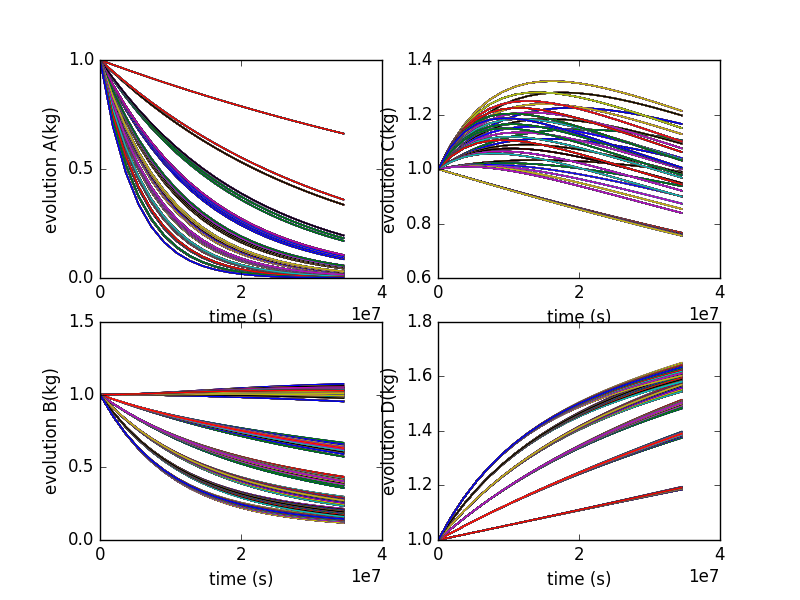
\includegraphics[scale=0.7]{pics/reducedOrderModelingHistoriesPhysicalModel.png}
  \caption{Plot of the histories generated by the Grid method for variables $A,B,C,D$.}
  \label{fig:ROMgrid_histories}
 \end{figure}
   %%%%%%%%%%%%%%%%%%%%%%%%%%%%%%%%%%%%%%%%%%%%%%%%%%%%%%%%%%
 %figure samples
 \begin{figure}[h!]
  \centering
  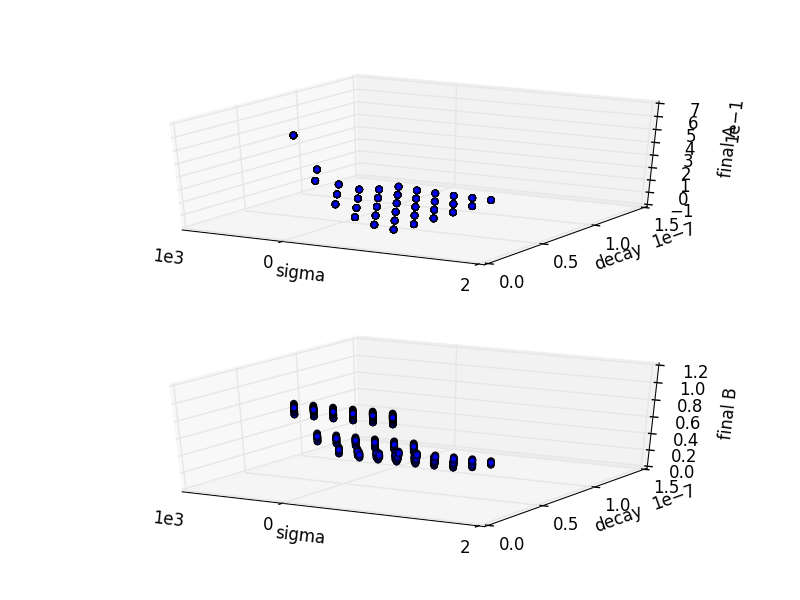
\includegraphics[scale=0.7]{pics/samplesPlot3DROMgp_scatter-scatter.png}
  \caption{Plot of the samples generated by the Grid sampling applied on the Gaussian Process ROM for variables $A,B$}
  \label{fig:ROMgp_samples}
 \end{figure}
 %%%%%%%%%%%%%%%%%%%%%%%%%%%%%%%%%%%%%%%%%%%%%%%%%%%%%%%%%%
 %%%%%%%%%%%%%%%%%%%%%%%%%%%%%%%%%%%%%%%%%%%%%%%%%%%%%%%%%%
   Finally, all the previously defined \textbf{Entities} can be combined in
   the \xmlNode{Steps} block. As inferable,
   eight \xmlNode{Steps} have been inputted:
   \begin{itemize}
     \item \xmlNode{MultiRun} named ``sample'', used to run the multiple
     instances of the driven code and
     collect the outputs in the two \textit{DataObjects}. As it can be
     seen, the \xmlNode{Sampler} is inputted to communicate to the
     \textit{Step} that the driven code needs to
     be perturbed through the Grid sampling strategy;
     \item \xmlNode{RomTrainer} named ``trainROMGaussianProcess'', used to construct (``train'')
     the GP ROM, based on the data-set generated in the  ``sample'' \textbf{Step};
     \item \xmlNode{RomTrainer} named ``trainROMsvm'', used to construct (``train'')
     the SVM ROM, based on the data-set generated in the  ``sample'' \textbf{Step};
     \item \xmlNode{RomTrainer} named ``trainROMinverse'', used to construct (``train'')
     the IDW ROM, based on the data-set generated in the  ``sample'' \textbf{Step};
     \item \xmlNode{MultiRun} named ``sampleROMGaussianProcess'', used to run the multiple
     instances of the previously constructed GP ROM and
     collect the outputs in the PointSet \textit{DataObject}. As it can be
     seen, the same \xmlNode{Sampler} used for perturbing the original model is here used.
     \item \xmlNode{MultiRun} named ``sampleROMsvm'', used to run the multiple
     instances of the previously constructed Support Vector Machine ROM and
     collect the outputs in the PointSet \textit{DataObject}. As it can be
     seen, the same \xmlNode{Sampler} used for perturbing the original model is here used.
     \item \xmlNode{MultiRun} named ``sampleROMInverse'', used to run the multiple
     instances of the previously constructed Inverse Distance Weight ROM and
     collect the outputs in the PointSet \textit{DataObject}. As it can be
     seen, the same \xmlNode{Sampler} used for perturbing the original model is here used.
     \item  \xmlNode{IOStep} named ``writeHistories'', used to 1) export
     the ``histories'' and ``samples''  \textit{DataObjects}
     \textbf{Entity} in a CSV file and 2) plot the responses of the sampling performed on the physical model, GP ROM,
     SVM ROM and IDW ROM in  PNG files and on the screen.
   \end{itemize}
\end{enumerate}

  %figure samples
 \begin{figure}[h!]
  \centering
  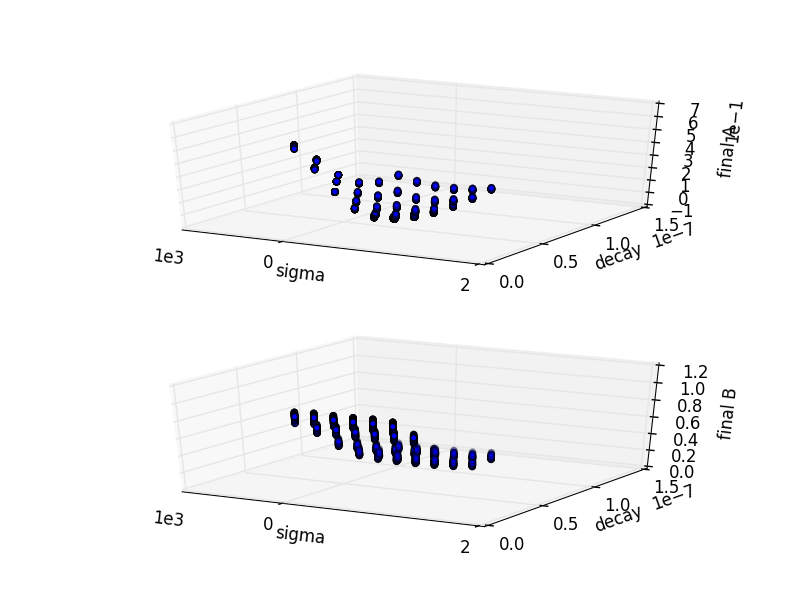
\includegraphics[scale=0.7]{pics/samplesPlot3DROMsvm_scatter-scatter.png}
  \caption{Plot of the samples generated by the Grid sampling applied on the Support Vector Machine ROM for variables $A,B$}
  \label{fig:ROMsvm_samples}
 \end{figure}
 %%%%%%%%%%%%%%%%%%%%%%%%%%%%%%%%%%%%%%%%%%%%%%%%%%%%%%%%%%
  %%%%%%%%%%%%%%%%%%%%%%%%%%%%%%%%%%%%%%%%%%%%%%%%%%%%%%%%%%
  %figure samples
 \begin{figure}[h!]
  \centering
  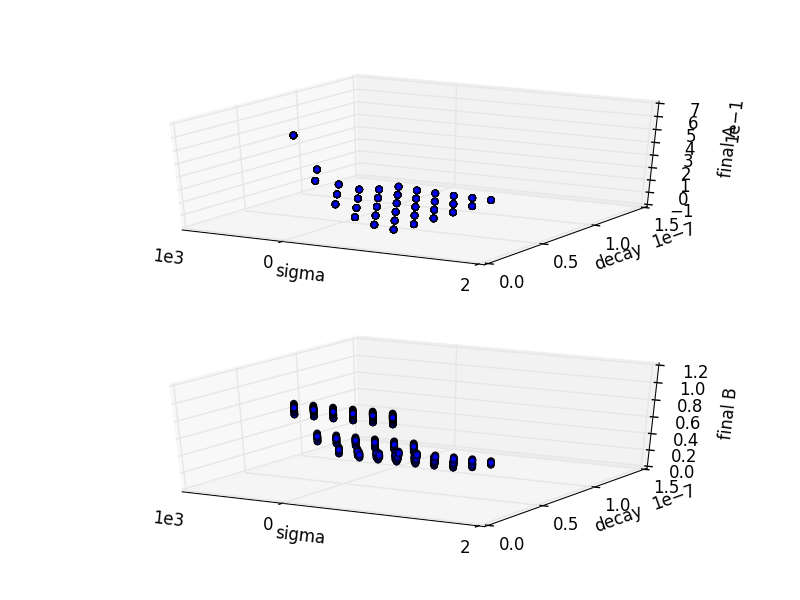
\includegraphics[scale=0.7]{pics/samplesPlot3DROMinverse_scatter-scatter.png}
  \caption{Plot of the samples generated by the Grid sampling applied on the Inverse Distance Weight ROM for variables $A,B$}
  \label{fig:ROMinverse_samples}
 \end{figure}
 %%%%%%%%%%%%%%%%%%%%%%%%%%%%%%%%%%%%%%%%%%%%%%%%%%%%%%%%%%
 Figure \ref{fig:ROMgrid_histories}
 shows the evolution of the outputs $A,B,C,D$ under uncertainties.
 Figure \ref{fig:ROMgrid_pointsets} shows the final responses  of $A and B$
 of the sampling employed using the driven code.

Figures \ref{fig:ROMgp_samples}, \ref{fig:ROMsvm_samples} and \ref{fig:ROMinverse_samples}  show the final responses  of $A and B$ of the sampling employed using the Gaussian Process, Support Vector Machines and Inverse Distance Weight ROMs, respectively.
It can be clearly noticed that the responses of the ROMs perfectly match the outcomes coming from the original model (see Figure   \ref{fig:ROMgrid_pointsets}).








